\documentclass{beamer}

\usepackage{amsmath}
\usepackage{amssymb}
\usepackage{booktabs}
\usepackage{hyperref}
\usepackage{rotating}
\usepackage{multirow}
\usepackage{colortbl,color}
\usepackage{graphicx}

\usepackage{tikz}

\defbeamertemplate{itemize subitem}{dash}{--}
\defbeamertemplate{itemize subsubitem}{dash}{--}
\setbeamertemplate{itemize item}[circle]
\setbeamertemplate{itemize subitem}[dash]
\setbeamertemplate{itemize subsubitem}[dash]
\setbeamertemplate{enumerate item}{\arabic{enumi}.}
\setbeamertemplate{enumerate subitem}{(\alph{enumii})}
\usefoottemplate{}

\newcommand{\showOn}[3]{\only<#2>{\color<#2>{black} #1}\only<#3>{\color<#3>{white} #1}}

\setbeamertemplate{headline}{}
\usenavigationsymbolstemplate{}
\setbeamercolor{titlelike}{fg=black}
\setbeamercolor{item}{fg=black}

\setbeamertemplate{background}{\tikz[overlay,remember picture]\node[opacity=0.2]at ([xshift=-0.075\textwidth,yshift=-0.075\textwidth]current page.north east){\includegraphics[width=0.1\textwidth]{bin/pittLogo}};}




\begin{document}
\title{\LARGE Econ 3610: Experimental Economics \\ Introductory Lecture}
\author{Alistair J. Wilson }
\date{Fall 2020}

\maketitle

\begin{frame}{Introduction [from Shadish, Cook, and Campbell]}

The increased emphasis on experimentation in the 16th and 17th centuries
marks the emergence of modern science from its roots in natural philosophy.

The scientific revolution departed in three ways from the common use of
observation in natural philosophy:
\end{frame}

\begin{frame}
\textbf{Departure 1:}

Increasingly used observation to correct errors in theory.

\

\pause
(As opposed to the use of observation to support one's own theory. Or
to the complete absence of observations and reliance on ``first principles,''
starting points known to be true by our nature or by divine revelation.)
\end{frame}

\begin{frame}
\textbf{Departure 2:}

Before the 17th century, appeals to experience were usually based on
passive observation of ongoing systems rather than on observation of what
happens after a system is deliberately changed.

\

\pause
After the scientific revolution the word experiment came to connote taking a deliberate action
followed by systematic observation of what occurred afterward.
\pause

\

Of Francis Bacon:
\begin{quotation}
He taught that not only must we observe nature in the raw, but that we must also `twist the lion's tail,' that is, manipulate our world in order to learn its secrets.\footnote{Anecdotally, Bacon may have died after contracting pneumonia while experimenting on the freezing of meat!}
\end{quotation}
\pause

\

Experimental science becomes concerned with observing the effects of manipulations.
\end{frame}



\begin{frame}
\textbf{Departure 3:}

Early experimenters realized the desirability of controlling
extraneous influences that might limit or bias observation.

\pause

\

Scientist carry telescopes to higher points, build laboratories, use sterilized equipment, take multiple observations.

\

When Social Scientists begin experimenting find it harder to use these same controls. Develop random assignment (Fisher) and control groups (Coover \& Angell).
\end{frame}

\begin{frame}
% http://en.wikipedia.org/wiki/Causality

\begin{center}
 \LARGE  What Are We Looking For?  \pause

 \textbf{Cause} $\Rightarrow$   \textbf{Effect}
\end{center}
\end{frame}

\begin{frame}{What Are We Looking For?  i) Cause.}
% http://en.wikipedia.org/wiki/Causality
\textbf{Cause}:

N. 1. a. The producer of an effect, result, or
consequence. b. The one, such as a person, an event, or a condition, that is
responsible for an action or a result.

V. 1. To be that cause of or reason
for; result in.
2. To bring about or compel by authority or force.
\end{frame}

\begin{frame}{Inus Condition}
Often what we refer to as a cause is an \textbf{INUS condition}:

an insufficient but non-redundant part of an unnecessary
but sufficient condition.

[cf.  J. L. Mackie (Australian philosopher who did some work on Metaphysics)
\end{frame}

\begin{frame}{INUS Condition Example}
\begin{itemize}
	\item A space-heater next to some curtains might \textbf{cause} a house-fire. \pause
	\item It is \textbf{insufficient}, because we also need oxygen, etc. \pause
	\item It is \textbf{non-redundant} part of a \textbf{sufficient} condition because without the space heater there'd be no fire \pause
	\item It is \textbf{unnecessary}, because house-fires occur in homes without space-heaters
\end{itemize}
\end{frame}

\begin{frame}{INUS Condition More Formal Example}
$$ \left(A \cap B \cap C\right)  \cup \left(W \cap  U\right) \cup \left(V\cap X \cap Y \cap Z\right)\Leftrightarrow E $$
\begin{itemize}
	\item A particular feature $A$ may be related to the effect $E$
	\item Insufficient as needs to be combined with $B$ and $C$
	\item Non-redundant as $B \cap C$ does not imply $E$ on its own
	\item Unnecessary as $W \cap U$ or $V\cap X \cap Y \cap Z$ also produce $E$ \pause
	
	\item \textbf{While it would be great to uncover the overall picture $E$, our attempts are frequently just to tease out small parts of a complex overall relationship}
\end{itemize}
\end{frame}


\begin{frame}{What Are We Looking For? ii) Effect.}\pause
A \textbf{counterfactual} is something that is contrary to fact. In an
experiment we observe what \textbf{did} happen when people received a treatment. The
counterfactual is knowledge of what would have happened to those same people
if they simultaneously had not received treatment. (cf. Hume below, but see Lewis, 1973 for more formal treatment)

\begin{quotation}
[W]here, if the first object had not been, the second never had existed.
\end{quotation}\pause

An \textbf{effect} is the difference between what did happen and what would
have happened.
\end{frame}

\begin{frame}{But...}
We cannot actually observe a counterfactual.\pause

\

A central task for all cause-probing research is to create reasonable
approximations to this physically impossible counterfactual.\pause

\

Through treatments and randomized assignment, we attempt to approximate counter-factuals.
\end{frame}


\begin{frame}{Causal Relationship}
A \textbf{causal relationship} exists if [according to John Stuart Mill]
\begin{enumerate}
\item The cause \textbf{preceded} the effect
\item The cause was \textbf{related} to the effect
\item We can find \textbf{no plausible alternative explanation} for the effect other than the
cause.
\end{enumerate}
\pause
In an experiment we:
\begin{enumerate}
\item Manipulate the presumed cause, and observe the ensuing effect.\pause
\item We see whether variation in the cause is related to variation in the effect.\pause
\item We try to reduce the plausibility of other explanations
\end{enumerate}

% http://www.philosophypages.com/lg/e14.htm A System of Logic
% http://en.wikipedia.org/wiki/Mill%27s_Methods
% A system of logic http://books.google.com/books?id=y4MEAAAAQAAJ and http://books.google.com/books?id=z4MEAAAAQAAJ
\end{frame}

\begin{frame}{From The Lab To The World}
The strength of experimentation is its ability to illuminate causal
inference.
\pause

\

But the weakness of experimentation is the doubt about the extent to which that
causal relationship generalizes.\pause

\

Experiments do very well at providing causal description (that there is a relationship) but not causal explanation (the why of the relationship).
\end{frame}

\begin{frame}{Generalization problems}
\begin{enumerate}
\item Construct Validity: causal generalization as Representation
    \begin{itemize}
        \item Did your study/experiment actually isolate what you think it does?
    \end{itemize}
\item External Validity: causal generalization as Extrapolation.
    \begin{itemize}
        \item Are the effects found in your study/experiment useful for explaining effects outside your setting?
    \end{itemize}
\end{enumerate}
\end{frame}


\begin{frame}{Generalization problems}
Theory can help us with this extrapolation, and attempt to give us causal explanations.

\

Experiments can be used to test select elements of a theory. Note however, that if we want a causal explanation, we must match \textbf{all} elements on the theory's predictions. Being right on a prediction for the wrong reasons is not explanatory.
\end{frame}

\begin{frame}{Testing theory}
Some of the (earlier) experimental literature tests the theory by verifying
the following quantitative prediction:
$$\text{Theoretical prediction}-\text{Average in data}\longrightarrow^p 0.$$

\pause
In general this is not a very fruitful approach because:
	\begin{enumerate}
		\item In a strict sense the theory is wrong unless the data was degenerate.
		\item Doesn't answer the more-qualitative question: are the forces at work in the model the
		ones at play in the data. (Theory as an approximation.)
	\end{enumerate}
\end{frame}

\begin{frame}{Testing theory: Smith's Precepts}
One way to deal with point 2 is to test qualitative (i.e directional) comparative-static predictions from the
theory with respect to the key variables of interest.

\

Smith (1982) defines conditions which are sufficient to allow for a
controlled testing of \textbf{economic} theories. \pause

The precepts are:
\begin{enumerate}
\item non-satiation
\item saliency
\item dominance
\item privacy.
\end{enumerate}
\end{frame}

\begin{frame}{Smith's Precepts}
\textbf{Non-satiation}:
\begin{quotation}
Given a costless choice between two alternatives, identical (i.e. equivalent) except that the first yields more of a reward medium (for example, US currency) than the second, the first will always be chosen (i.e. preferred) over the second, by an \emph{autonomous} individual. Hence utility, $U(V)$, is a monotone increasing function of the monetary reward, $U'>0$, where $V$ is dollars of currency.
\end{quotation}
\end{frame}

\begin{frame}{Smith's Precepts}
\textbf{Saliency}:
\begin{quotation}
Individuals are guaranteed the right to claim a reward which is increasing (decreasing) in the good (bad) outcomes, $x_i$, of an experiment; individual property rights in messages, and how messages are to be translated into outcomes are defined by the institution of the experiment
\end{quotation}
\pause

Effectively, this is stating that the relationship between final outcomes (the payoffs), and the the actions taken (the ``messages'') are understood by the subjects.
\end{frame}

\begin{frame}{Smith's Precepts}
\textbf{Dominance}:
\begin{quotation}
The reward structure dominates any subjective costs (or values) associated with participation in the activities of an experiment.
\end{quotation}
\pause

	\begin{itemize}
		\item This ensures that the experimenter has not lost control of the preferences
		\item We can do this by paying more, or by making the experiment clearer
	\end{itemize}
\end{frame}

\begin{frame}{Smith's Precepts}
In many early studies, \textbf{subjects were not paid}.

This leads to the failure of Precepts 1 to 3.

Nonetheless, results were not typically different from the follow up experiments where subjects were paid!
\end{frame}

\begin{frame}{Smith's Precepts}
\textbf{Privacy}:
\begin{quotation}
Each subject in an experiment is given only information on his/her own payoff alternatives.
\end{quotation}
\pause

	\begin{itemize}
		\item If you are interested in altruistic preferences, note that information about others' payoffs is therefore included in the above definition
		\item We might want to stop subjects engaging in a tournament, unrelated to payoffs
		\item Note that in most games, information on others' potential payoffs is necessary to understand your own payoffs
	\end{itemize}
\end{frame}


\begin{frame}{Testing theory: Smith's Precepts}
The previous four precepts ensure the internal validity.
A fifth precept, \textbf{Parallelism} make experimental results transferable (this is effectively external validity).

\begin{quotation}
	Propositions about the behavior of individuals and the performance of institutions that have been tested in laboratory microeconomies apply also to non-laboratory microeconomies where similar \emph{ceteris paribus} conditions hold.
\end{quotation}

\pause

Is the theory induced in the lab relevant to the external setting.
\end{frame}

\begin{frame}{Parallelism}

\begin{quotation}
	The appropriate way to falsify parallelism with respect to some particular aspect of behavior is to show that some replicable property of a theory or institution in a laboratory microeconomy is falsified with field data ... such studies are welcome, and are necessary, if answers of substance are to be provided to questions of parallelism
\end{quotation}

\end{frame}

\begin{frame}{Parallelism}
Smith:
\begin{quotation}
	In terms of the evidential standards and precedents that have been established in this literature, it is not appropriate to list reasons why experimental subjects \emph{might} be different from what one imagines \emph{might} be important about ``real world'' behavior. Speculating about a list of differences between two microeconomies is not the same thing as showing empirically that the microeconomies exhibit different behavior and that this is because of factors appearing in the list.
\end{quotation}

And when we do find empirical differences in behavior between the lab and field, the better questions to ask are: Why is there a difference? Why did parallelism fail?

\end{frame}


\begin{frame}{Types of Experimental Paper}
Schotter (2008) breaks experiments on economic theory into two broad categories\pause

\begin{itemize}
	\item Structural
	\item Comparative Statics
\end{itemize}

\end{frame}

\begin{frame}
\begin{itemize}
	\item Structural tests seem more useful when dealing with \textbf{Explanatory} theories or when considering policy with the need for estimated parameters.
	\begin{itemize}
		\item Assuming the theory is true, what parameter best fits the observed data
		\item For example: risk parameters, temporal substitution
	\end{itemize}
	\item Comparative Static tests are used in both a strong and weak form as \textbf{tests} of whether the theory is true (so there needs to be some potential to falsify it):
	\begin{itemize}
		\item Does the data match the comparative-static predictions of the theory. In direction? In levels?
	\end{itemize}
\end{itemize}

\end{frame}
\begin{frame}{Hurlbert's problems and solutions}
Given some of the similarities between economic experiments and ecological experiments (which have a deeper history), let's look at some of design features used to solve problems that arise in field ecology in Hurlbert, Stuart H. (1984) ``Pseudoreplication and the Design of Ecological Field
Experiments,'' Ecological Monographs, 54:2, pp. 187-211.
\end{frame}


\begin{frame}{Potential sources of confusion in an experiment}
\small
\begin{tabular}{p{0.4\textwidth}cp{0.5\textwidth}}\toprule
\textbf{Source of confusion} &  & \textbf{Design features to address}\\\midrule
 Temporal change  & & Control   treatments \\\midrule
 Procedure effects  & & Control   treatments \\\midrule
 Experimenter bias & & Randomized  assignment \\
 & & Randomization of  conduct\\
 & & ``Blind'' procedures \\\midrule
 Experimenter-generated  & & Replication of treatments \\
 variability & & \\ \midrule
 Experimental-unit  & & Replication of treatments\\
 variability & & Interspersion of treatments\\
  & & Concomitant  observations\\ \midrule
  Non-demonic intrusion & & Replication of   treatments\\
   & & Interspersion of treatments\\ \midrule
 Demonic intrusion & & Eternal vigilance, exorcism, \\& & human sacrifices, etc.\\ \bottomrule
\end{tabular}
\end{frame}

\begin{frame}{Demonic Intrustion}
Explaining what he means, Hurlbert writes:
\begin{quotation}
If you worked in areas inhabited by demons you would be in
trouble regardless of the perfection of your experimental designs. If a
demon chose to ``do something'' to each
experimental unit in treatment A but to no experimental unit in treatment B,
and if his/her/its visit went undetected, the results would be misleading.
One might also classify the consequences of certain design or execution
errors as demonic intrusion. \pause For example, if effects of fox predation are
studied using fenced and unfenced fields, hawks, may be attracted to the
fence posts and use them as perches from which to search for prey. Later,
foxes may get credit for treatment effects generated in the fenced fields by
the hawks.
\end{quotation}
\pause
Until you have a model of hawk behavior, your methodology cannot
appropriately isolate the effect of fencing on fox predation.
\end{frame}

\begin{frame}{Demonic Intrustion}

\begin{quotation}
Whether such non-malevolent entities are regarded as
demons or whether one simply attributes the problem
to the experimenter's lack of foresight and the inadequacy
of procedural controls is a subjective matter. It
will depend on whether we believe that a reasonably
thoughtful experimenter should have been able to foresee
the intrusion and taken steps to forestall it.
\end{quotation}
\end{frame}

\begin{frame}{Practical Considerations for Experimental Design}
	\begin{enumerate}
		\item Instructions and Information
		\item Subject Characteristics
		\item End-game Rules and Equilibria
		\item Payoffs and Parameters
		\item Factorial Design
		\item Statistical Tests
	\end{enumerate}
\end{frame}

\begin{frame}{Instructions and Information}
	\begin{itemize}
		\item What should be common knowledge?
		\item What should be private information?
		\item How much calculation help should we provide?
		\item What type of language should we use?
		\item What type of coaching, if any, should subjects receive?
	\end{itemize}
\end{frame}

\begin{frame}{Instructions and Information}
	\begin{itemize}
		\item Instructions will define your experimental results and subsequently your paper
		\item Care should be taken with every word and phrase.
		\item In general, we should be careful with labels:
			\begin{itemize}
				\item Labels may affect subjects differently and activate heuristics
				\item This subjectivity is a loss of control on the subject's motives
				\item Keep control and focus on the economic incentives
			\end{itemize}
	\end{itemize}
\end{frame}

\begin{frame}{Instructions and Information: Common vs Private}
	\begin{itemize}
		\item Common Knowledge is (hopefully) achieved by reading instructions aloud
		\item Private Knowledge is achieved by providing subjects with information on their private screens\pause
		\item Normally the theory we are testing will explicitly tell us what is and is not private knowledge
		\item Subject's parameters are quite frequently private knowledge, but knowledge of the distribution of these parameters frequently needs to be common knowledge
		\item Subject identities are normally masked
		\item Per Smith, subjects collective earnings are normally only shown to the specific subject
	\end{itemize}
\end{frame}

\begin{frame}{Instructions and Information: Calculation Aids}
	\begin{itemize}
		\item A theory might fail because:
		\begin{enumerate}
			\item The equilibrium theory works but subjects cannot perform the calculations required
			\item Subjects are perfect calculators, but the equilibrium theory does not work
		\end{enumerate}\pause
		\item If we think the first failure type likely, then we do not want to give calculation aids in all treatments, as this is what we would like to test
		\item But, in the second we would want to isolate the failure of the theory by providing calculation aids
		\pause
		\item Where calculation aids are useful is for understanding base-level preferences, I normally err on providing help
	\end{itemize}
\end{frame}

\begin{frame}{Subject Characteristics}
	\begin{itemize}
		\item Should subjects be pre-tested and sorted according to characteristics?
		\item Should experienced subjects be used, and if so should they be mixed with experienced subjects?
		\item Should subjects from student populations be used or another special population?
		\item Should subjects stay in fixed roles or rotate roles?
		\item How many times should a set of subjects perform the experiment?
		\item Should subjects face a variety of parameter values in succession?
		\item How many independent groups of subjects should perform the experiment?
	\end{itemize}
\end{frame}

\begin{frame}{Subject Characteristics: Undergraduates}
The good:
	\begin{itemize}
		\item Bright
		\item Know how to listen
		\item Want/Need Money
		\item Don't have too much baggage
	\end{itemize}\pause

The Bad:
	\begin{itemize}
		\item Wealthier than average
		\item Younger than average
		\item More educated than average
		\item Racially non-representative
	\end{itemize}
\end{frame}

\begin{frame}{Subject Characteristics: Special Subject Pools}
	\begin{enumerate}
		\item Allow substantive explanation of phenomena about groups
		\item Stability of parameter estimates across pools
		\item Professionals vs. Undergrads
		\item Questions that cannot be asked for non-human subjects
		\item Other (e.g. Children, ex-post observation)
	\end{enumerate}
\end{frame}

\begin{frame}{Subject Characteristsics: Populations}
\tiny
	\begin{itemize}
		\item Kagel, John H. (1987) ``Chapter 6: Economics according to the rats (and pigeons too): what have we learned and what can we hope to learn?'' in Laboratory experimentation in economics: six points of view, edited by Alvin E. Roth.
		\item Burns (1985) ``Experience And Decision Making: A Comparison Of Students And Businessmen In A Simulated Progressive Auction,'' in Research In Experimental Economics.
		\item DeJong, Forsythe, and Uecker (1988) ``A Note On The Use Of Businessmen As Subjects In Sealed Offer Markets,'' Journal of Economic Behavior \& Organization.
		\item Dyer, Kagel, and Levin (1989) ``A Comparison Of Naive And Experience Bidders In Common Value Offer Auctions: A Laboratory Analysis,'' The Economic Journal.
		\item Anderson and Shunder (1995) ``Professional Traders As Intuitive Bayesians,'' Organizational Behavior And Human Decision Processes.
		\item Cadsby and Maynes (1998) ``Choosing Between A Socially Efficient And Free-Riding Equilibrium: Nurses versus Economics And Business Students,'' Journal of Economic Behavior \& Organization.
		\item Cooper, Kagel, Lo, and Gu (1999) ``Gaming Against Managers In Incentive Systems: Experimental Results with Chinese Students and Chinese Managers,'' American Economic Review.
	\end{itemize}
\end{frame}

\begin{frame}{Subject Characteristics: Populations}
\tiny
	\begin{itemize}
		\item Potters and van Winden (2000) ``Professionals And Students In A Lobbying Experiment Professional Rules Of Conduct And Subject Surrogacy,'' Journal of Economic Behavior \& Organization.
		\item Fehr and List (2004) ``The Hidden Costs And Returns Of Incentives---Trust And Trustworthiness Among CEOs,'' Journal of the European Economic Association.
		\item Montmarquette, Rulliere, Villeval, and Zeiliger (2004) ``Redesigning Teams and Incentives In A Merger: An Experiment With Managers And Students,'' Management Science.
		\item Carpenter and Seki (2005) ``Do Social Preferences Increase Productivity? Field experimental evidence from fishermen in Toyama Bay,'' IZA DP No. 1697.
		\item Palacios-Huerta and Volij (2008) ``Experientia Docet: Professionals Play Minimax in Laboratory Experiments,'' Econometrica.
		\item Alevy, Haigh, and List (2006) ``Information Cascades: Evidence From A Field Experiment With Financial Market Professionals,'' The Journal of Finance.
	\end{itemize}
\end{frame}

\begin{frame}{Subject Characteristics: Populations}
Summary:
	\begin{itemize}
		\item Mixed Results.
		\item Many similarities but also many insightful differences
		\item Qualitatively, many results are very similar
	\end{itemize}
\end{frame}

\begin{frame}{End-Game Rules and Equilibria}
	\begin{itemize}
	\item How should the experiment end---what is the termination rule?
	\item Which observations are appropriate for statistical tests?
	\end{itemize}
\end{frame}

\begin{frame}{End-Game Rules and Equilibria}
	\begin{itemize}
		\item Theory is frequently for one-shot games (or one-run of a repeated game)
		\item But experiments are frequently dynamic games with multiple repetitions
		\item The theory for repeated games (or repeated-repeated-games) can be distinct \pause
		\item Solution:
    		\begin{itemize}
    			\item Random rematching (Stranger)
    			\item Turnpike design (Perfect Stranger)
    		\end{itemize}
	\end{itemize}
\end{frame}

\begin{frame}{End-Game Rules and Equilibria}
	\begin{itemize}
		\item Many experiments exhibit end-game effects
		\item Which period should we then use for testing? \pause
		\item Solution:
		\begin{itemize}
			\item Random termination
			\item Convergence termination
			\item Eyeballing and dropping terminal-effect rounds
		\end{itemize}
	\end{itemize}
\end{frame}

\begin{frame}{Payoffs and Parameters}
	\begin{itemize}
		\item How do we/should we calibrate payoffs?
		\item Should subjects play for money directly or for chips convertible into money?
		\item How should the problem of actual loses by subjects be treated?
		\item How do we decide upon the parameter values?
	\end{itemize}
\end{frame}

\begin{frame}{Payoffs and Parameters}
	\begin{itemize}
		\item Theories are typically point predictions
		\item But a lot depends on the shape of the payoff functions
		\item With some small noise in this payoff, what is the effect on the theory for each treatment?
		\item Large differences in the choice might have very small effects on final payoffs
		\item When we make changes across treatments should we:
		\begin{itemize}
			\item Keep total payoffs constant?
			\item Keep marginal incentives constant?
		\end{itemize}
	\end{itemize}
\end{frame}

\begin{frame}{Payoffs and Parameters}
	\begin{itemize}
		\item Frequently labs will have guidelines on expected payments 
		\item But we normally have to guarantee them some minimum amount for their time, and we are certainly not allowed to take money from the subjects 
		\item This has the effect to weaken our incentives if there are potential losses:
		\item Some potential solutions:
		\begin{itemize}
			\item Give endowment of wealth up front to suck up all potential losses
			\item Let subjects go bankrupt and drop out of experiment
			\item Find a ``last'' experimental round where everyone was doing well to wipe out losses.
		\end{itemize}
	\end{itemize}
\end{frame}

\begin{frame}{Payoffs and Parameters}
	\begin{itemize}
		\item Avoid constructing experiments where the equilibrium you are testing is too salient.
		\begin{itemize}
			\item Too central (e.g. 50 on a 0 to 100 interval)
			\item Boundaries (0 or 100), where this also leads to statistical problems
		\end{itemize}
	\item But at the same time we want to maximize the distance between predictions across treatments
	\end{itemize}
\end{frame}

\begin{frame}{Payoffs and Parameters}
	\begin{itemize}
		\item Many experiments will pay the sum of all rounds
		\item Each round has small payoff
		\item However, this might induce wealth effects whereby behavior changes over rounds dependent on the total earnings
		\pause
		\item I personally prefer paying a random round, where theory supports this (see Azrieli, Chambers and Healy, JPE 2018)
	\end{itemize}
\end{frame}

\begin{frame}{Factorial Design}
	\begin{itemize}
		\item Is a factorial design a prerequisite for a valid experiment or can less controlled experiments be informative?
	\end{itemize}
\end{frame}

\begin{frame}{Factorial Design}
Suppose we believe that the variable $z$ is affected by $x$ and $y$. And we look at 3 parameterizations of each variable.

\begin{center}
\only<2>{\begin{tabular}{r|ccc}
 & $x_1$ & $x_2$ & $x_3$ \\\hline
$y_1$ & $z(x_1,y_1)$ & $z(x_2,y_1)$  & $z(x_3,y_1)$  \\
$y_2$ & $z(x_1,y_2)$ & $z(x_2,y_2)$  & $z(x_3,y_2)$  \\
$y_3$ & $z(x_1,y_3)$ & $z(x_2,y_3)$  & $z(x_3,y_3)$  \\
\end{tabular}
}
\only<3>{\begin{tabular}{r|ccc}
 & $x_1$ & $x_2$ & $x_3$ \\\hline
$y_1$ & $z(x_1,y_1)$ & $z(x_2,y_1)$  & $z(x_3,y_1)$  \\
$y_2$ & $z(x_1,y_2)$ & $z(x_2,y_2)$  &   \\
$y_3$ & $z(x_1,y_3)$ &  & $z(x_3,y_3)$  \\
\end{tabular}
}
\only<4>{\begin{tabular}{r|ccc}
 & $x_1$ & $x_2$ & $x_3$ \\\hline
$y_1$ & $z(x_1,y_1)$ & $z(x_2,y_1)$  &   \\
$y_2$ & $z(x_1,y_2)$  & $z(x_2,y_2)$  & $z(x_3,y_2)$  \\
$y_3$ &  & $z(x_2,y_3)$  & $z(x_3,y_3)$  \\
\end{tabular}
}
\end{center}
\end{frame}

\begin{frame}{Statistical Tests}
\begin{itemize}
\item What types of statistical tests should be performed?
\end{itemize}
\end{frame}

\begin{frame}{Statistical Tests}
\begin{itemize}
\item Frequently this means what level will we aggregate over:
	\begin{itemize}
		\item Over subjects
		\item Over periods
		\item Over both
	\end{itemize}
\item I will talk in the next lecture about statistical tests/effects in more detail
\end{itemize}
\end{frame}

\begin{frame}{Aggregation of Data (Subject Average)}
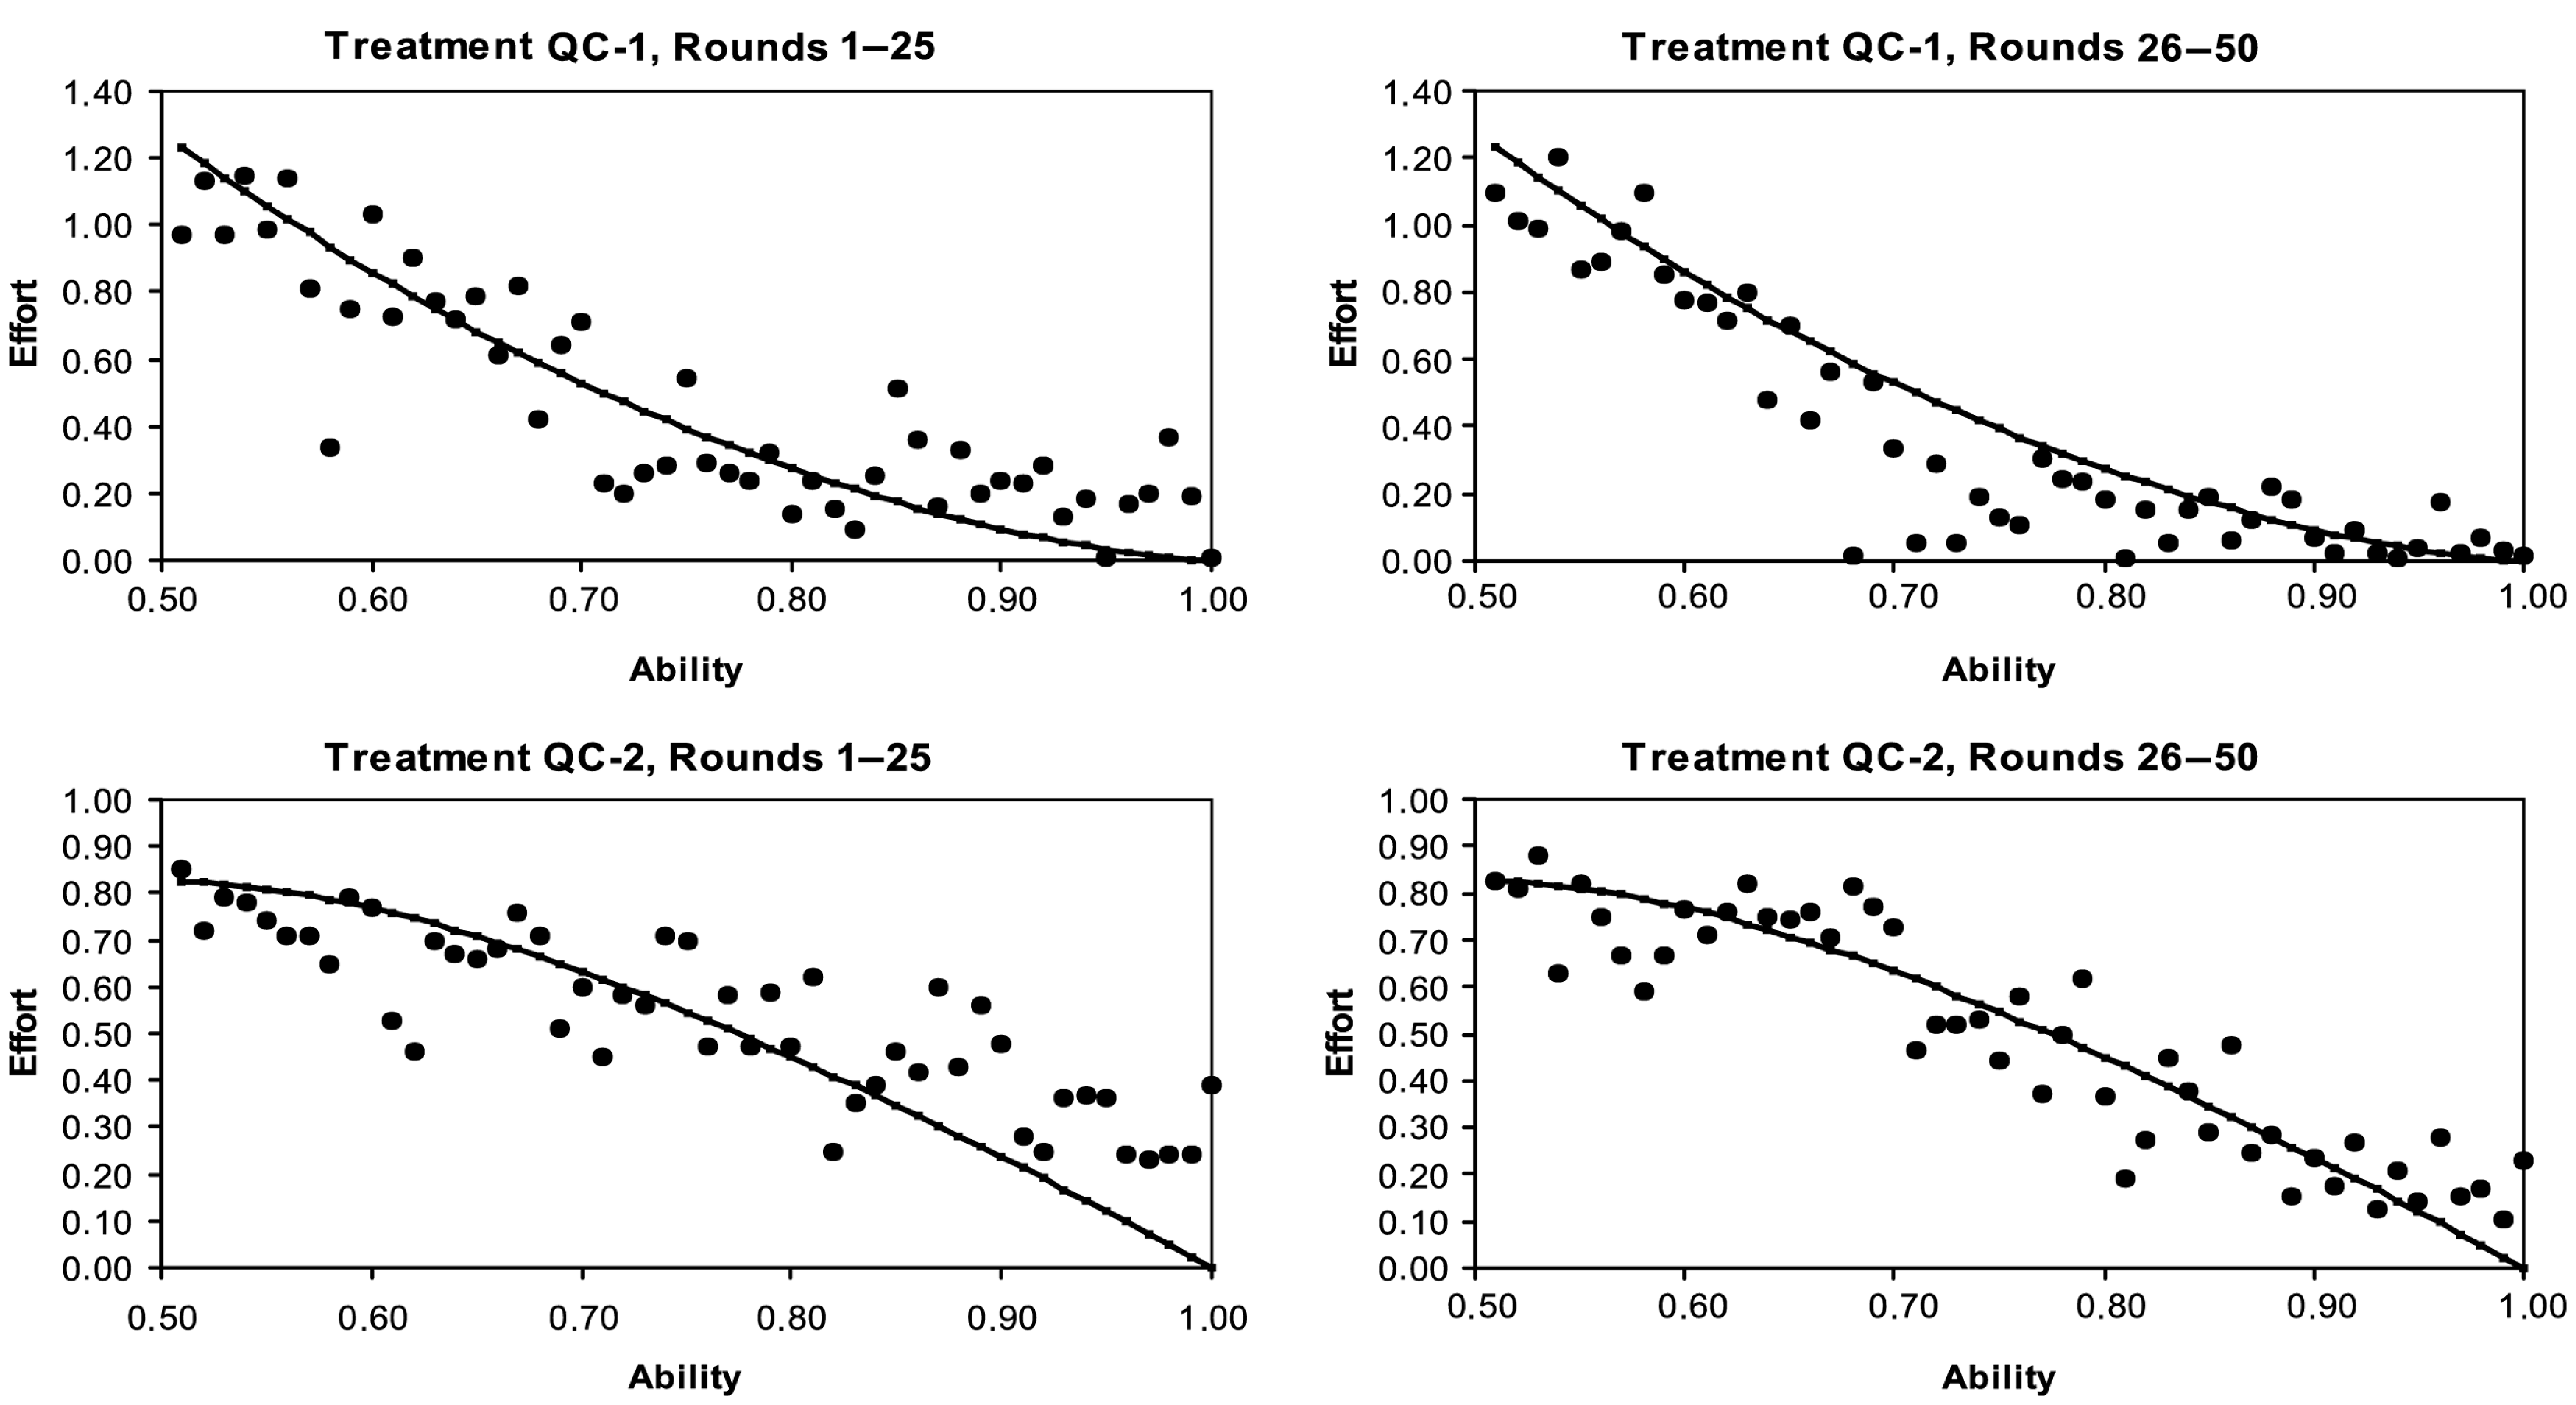
\includegraphics[width=1.0\textwidth]{./i/SchotterMueller1.eps}
\end{frame}
\begin{frame}{Aggregation of Data (Individual Subjects)}
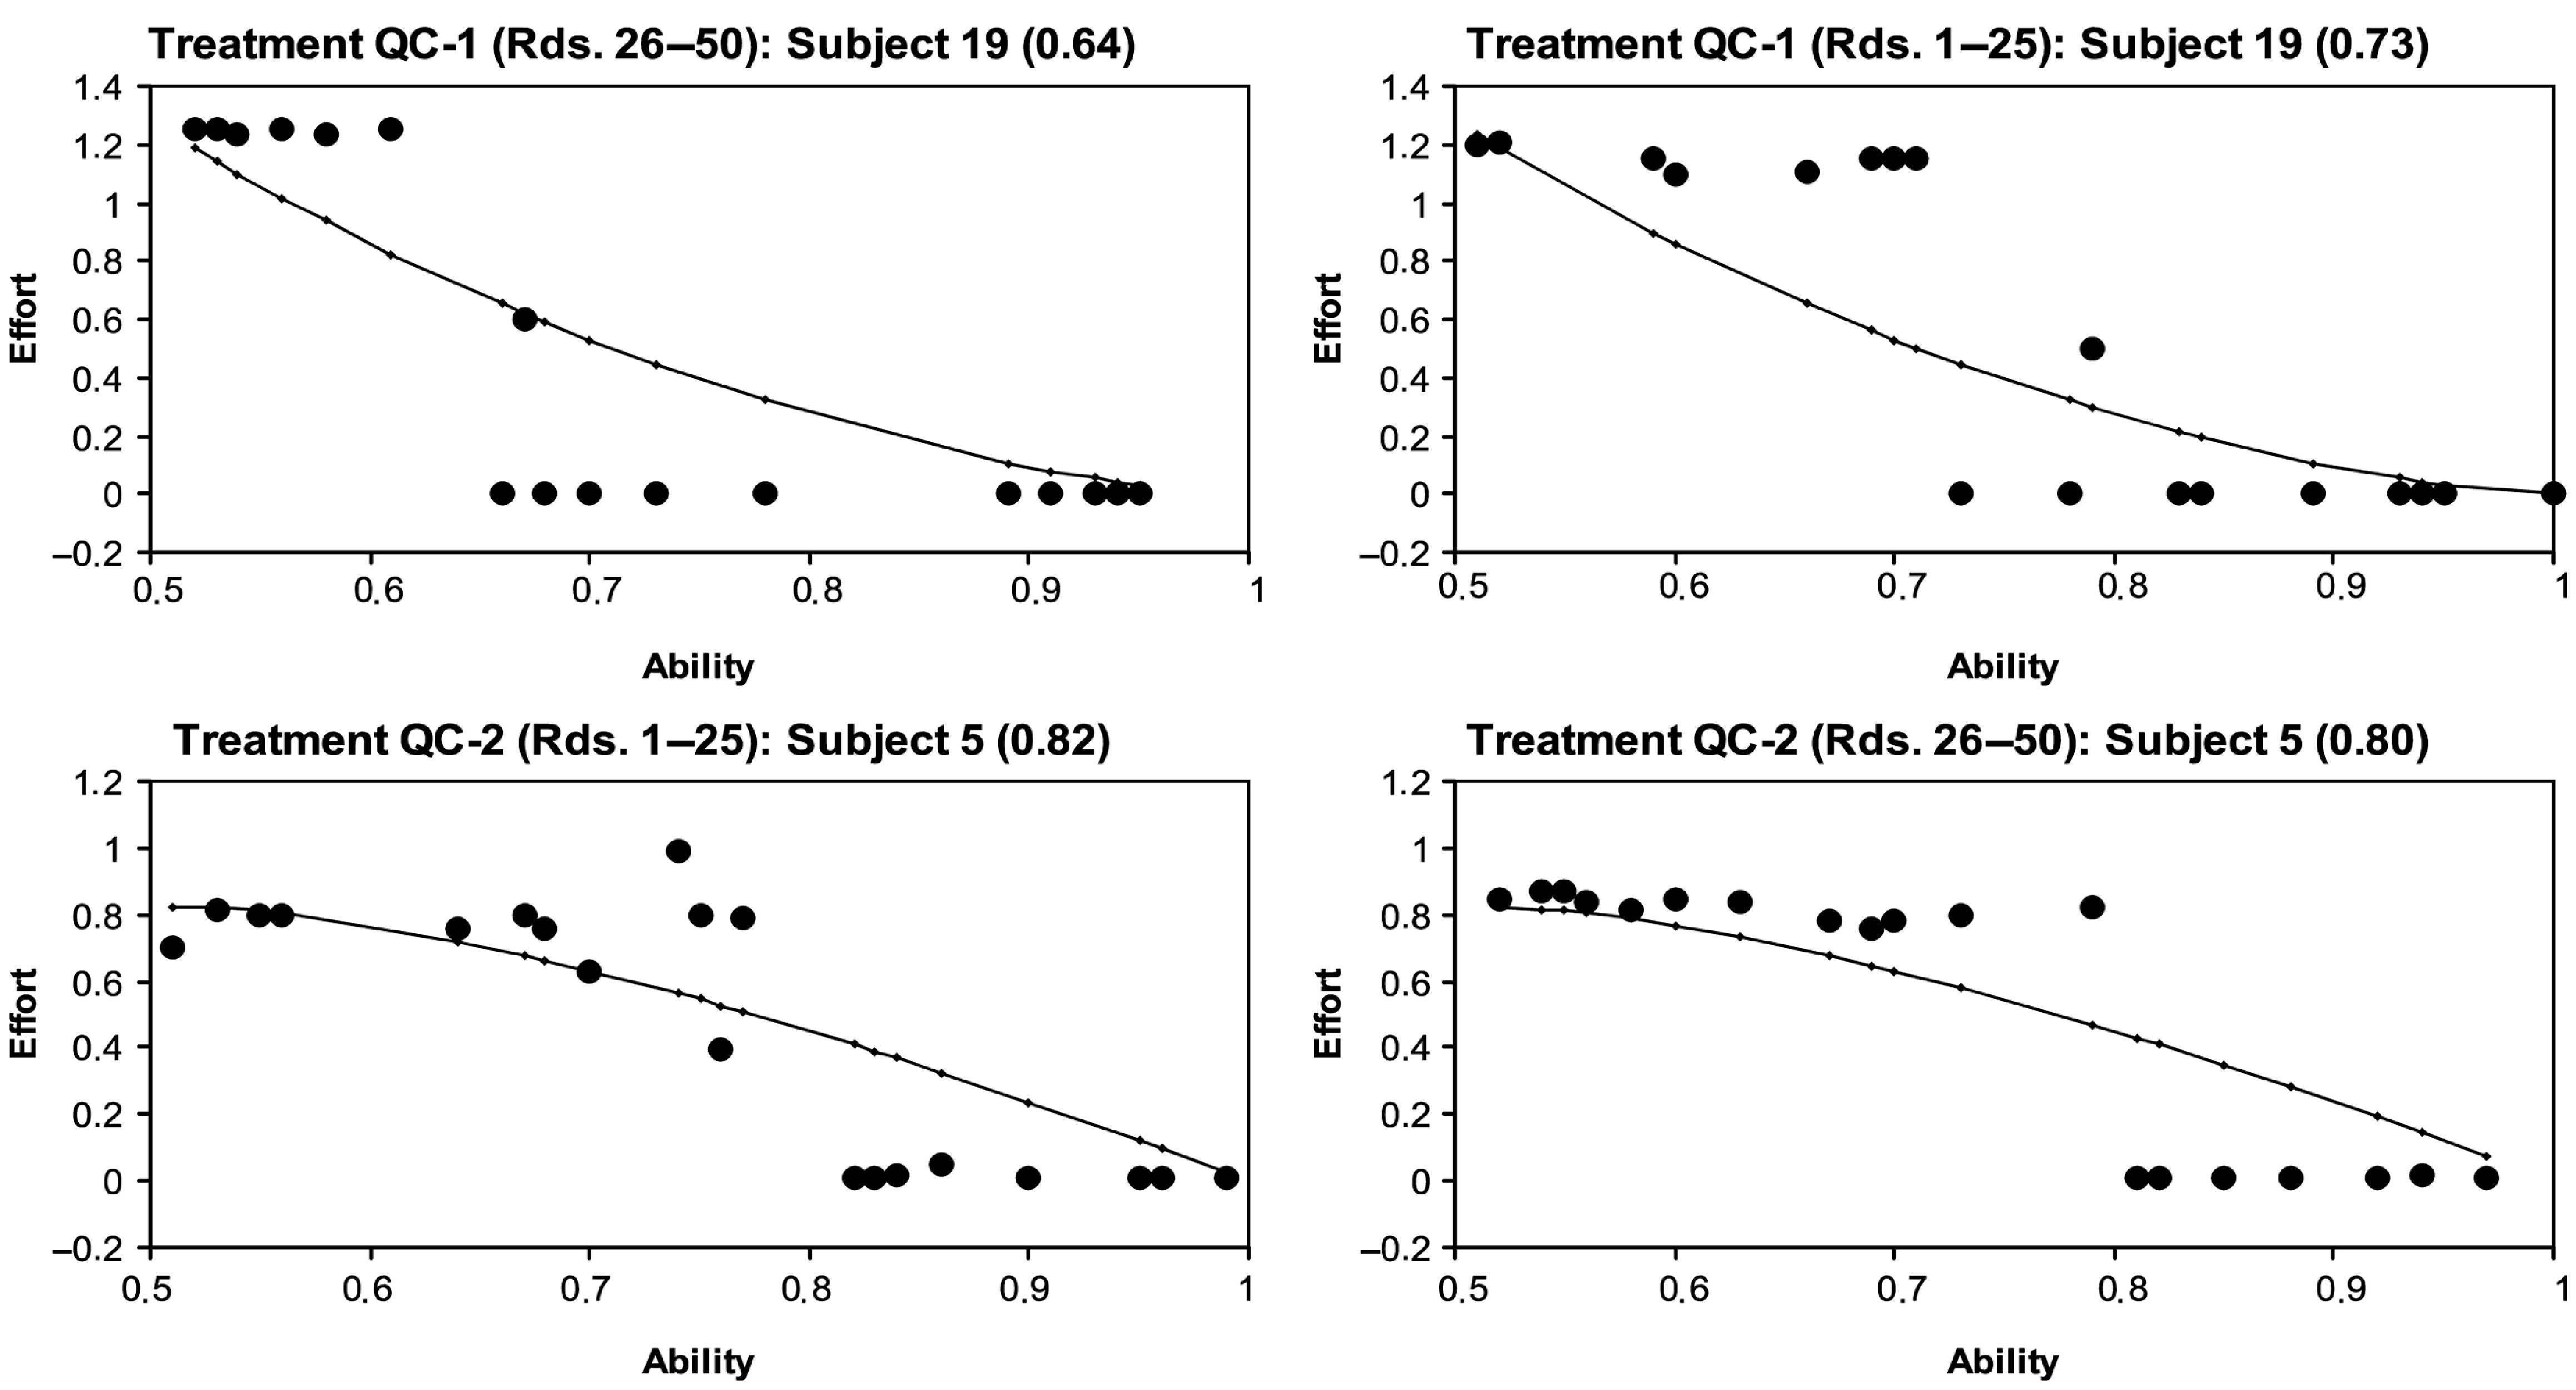
\includegraphics[width=1.0\textwidth]{./i/SchotterMueller2.eps}
\end{frame}

\end{document}
